\documentclass[a4paper,10pt]{article}
\usepackage[utf8]{inputenc}
\usepackage{graphicx}
\graphicspath{ {./code/} }

\title{\textbf{Coordination and Utility} \\ 
\textbf{Assignment III}}

\author{Emil Ståhl and Peyman Peirovifar}

\begin{document}

\maketitle
\textbf
{\\1. Introduction\\\\}
This report covers the implementation of a two tasks, the first is about positioning speakers at main stage (N Queen problem), and the second simulation is about visit all acts, minimize traveling time and crowd at acts. The aim of the first task is to understand how agents communicate and cooperate to achieve their goal using the N Queens problem. The second simulation gives hands on experience with agents working together to find a solution to a problem as well as agent utility function to control behavior. 

\maketitle
\textbf
{\\2. The program and its purposes\\\\}
The program consists of only one type of agent/species, the queen, (similar to classes in objective oriented programming).

\maketitle
\textbf
{\\2.1 Implementation of N Queens problem\\\\}
In the global scope of the model we initialize some variables, draw the chessboard and create the queens to be used later. Next the queens species is created with the skills of moving and FIPA communication. Variables are initialized for the species to use in its reflexes. The reflexes are moveToTarget, placeMe, requestParent and read\_request\_message. Additionally, there are one action moveTo and two boolean methods safeAt and moveToNextSafePosition.
The boolean method safeAt takes a position and evaluates if the position is safe, i.e. it does not share row or column with another queen. The other boolean method moveToNextSafePosition calculates a new position by passing to safeAt. Each queen holds a map / list of all position it has been placed at. So if the newly calculated has been visited previously or it is not safe the method return false. Otherwise it returns true if the position is new and safe.
The moveToNextSafePosition method is called from the placeMe reflex, depending on what the method returns it will trigger either to request the agents parent or set the isReady flag to true. The request to the parent is done thru FIPA. 

\begin{verbatim}
do start_conversation (to ::[parent], protocol:: 'fipa-request', 	
\end{verbatim}
\begin{verbatim}
performative:: 'request', contents::[self.name, "move-next"]
\end{verbatim}
Each agent also have the read\_request\_message reflex handling the FIPA requests. If the message received is ”move-next” it checks if it can move, if not it starts a conversation with it child to reset. If the message is ”reset-child” it clears its map of visited positions. This is sort of a backtracking technique.  

\maketitle
\textbf
{\\2.2 Implementation of visiting highest utility stage\\\\}
The simulation consists of four dance floors with different attributes. The attributes are Band, Lights, Sound, Dj Set, Vibe and Crowd and are rated from 1-10. Each visiting guest has its own preferences on which stage to visit. Every time an event starts, the dance floor informs all agents with the attributes of this specific event using the FIPA protocol. The agents compute the utility of each new event based on the event attributes and the agents’ preferences. With every new event the agent compares his current utility with the potential utility with visiting this new event, and acts accordingly. Since the attribute crowd changes over time, each agent requests the attributes from all active stages every 100 steps using the FIPA protocol, makes a new utility computation.

\clearpage
\maketitle
\textbf
{\\\\3. Results\\\\}
Shown below is part of the message log and a snapshot of the two simulations running. 

\maketitle
\textbf
{\\\\3.1 N Queens Problem\\\\}

\begin{verbatim}
Queen8: Received move-next request
Queen9: Finding a place
Queen9: Checking new position = 9
Queen9: Checking new position = 10
Queen9: Checking new position = 11
Queen9: Checking new position = 0
Queen9: Checking new position = 1
Queen9: Checking new position = 2
Queen9: Checking new position = 3
Queen9: Checking new position = 4
Queen9: Checking new position = 5
Queen9: Checking new position = 6
Queen9: Checking new position = 7
Queen9: Can not move, requesting parent
Queen9: Received move-next request
Queen10: Received move-next request
Queen11: Received move-next request
Queen8: Received move-next request
\end{verbatim}

\begin{center}{}
\centering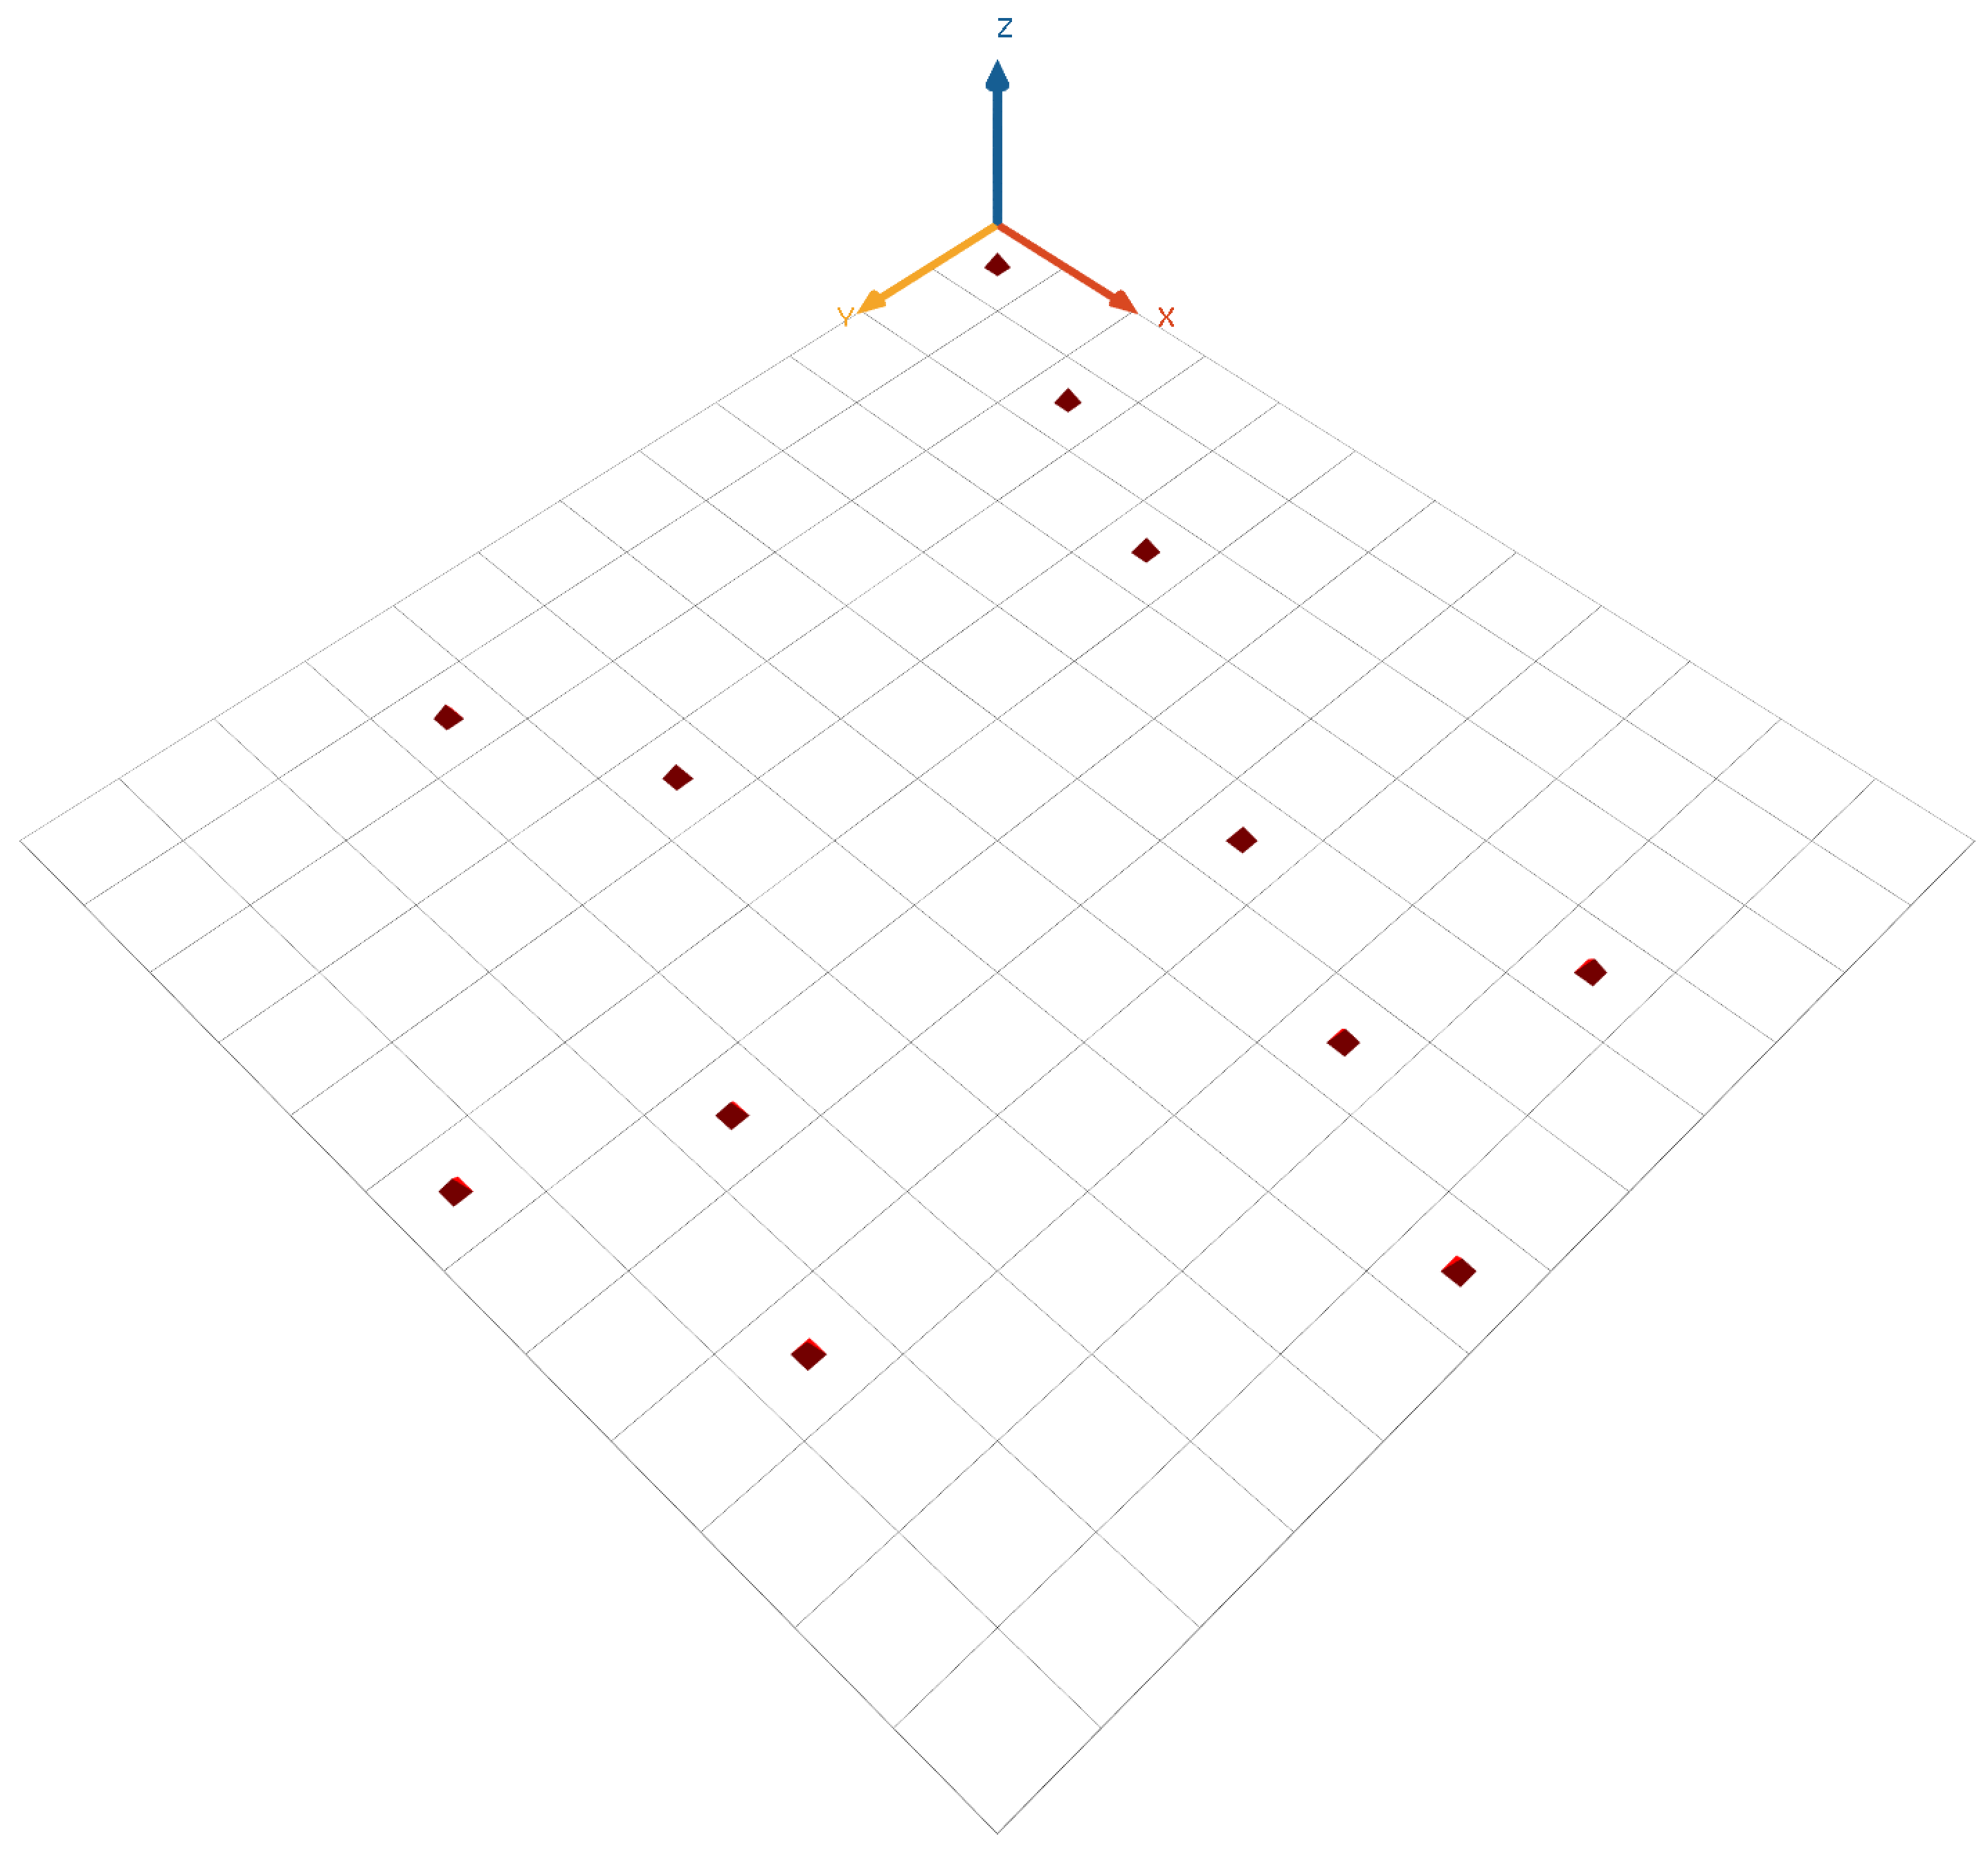
\includegraphics[scale=0.3]{Queen.png}\par
\end{center}

\clearpage
\maketitle
\textbf
{\\\\3.2 Visiting highest utility stage\\\\}

\begin{center}{}
\centering\includegraphics[scale=0.3]{Festival.png}\par
\end{center}


\maketitle
\textbf
{\\\\4. Conclusions\\\\}
This work gave more experience working with Agents and how they communicate and cooperate in order to achieve their goals. Additionally, the utility function for controlling behavior was implemented in a real world implementation.
\end{document}
